\begin{figure}[htbp]
\section*{AIRE}
\centering
\begin{subfigure}[b]{0.95\textwidth}
\centering
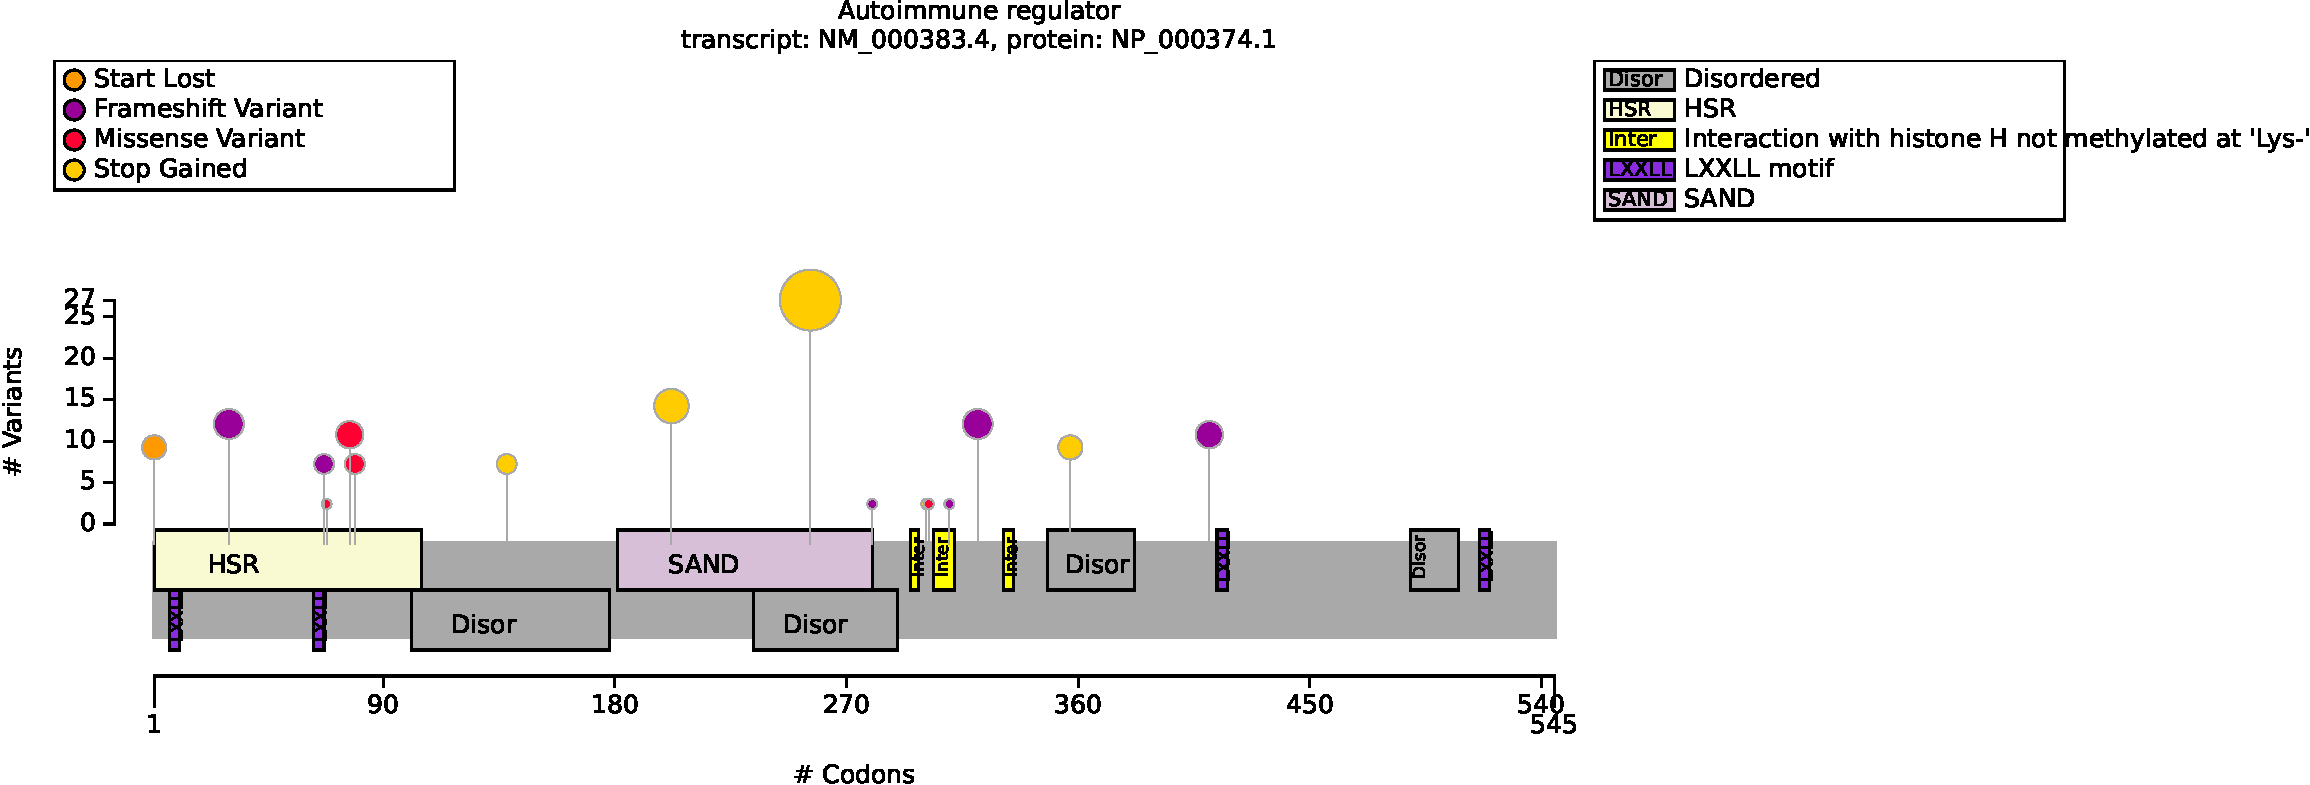
\includegraphics[width=\textwidth]{ img/AIRE_protein_diagram.pdf} 
\captionsetup{justification=raggedright,singlelinecheck=false}
\caption{Distribution of variants in AIRE}
\end{subfigure}

\vspace{2em}

\begin{subfigure}[b]{0.95\textwidth}
\centering
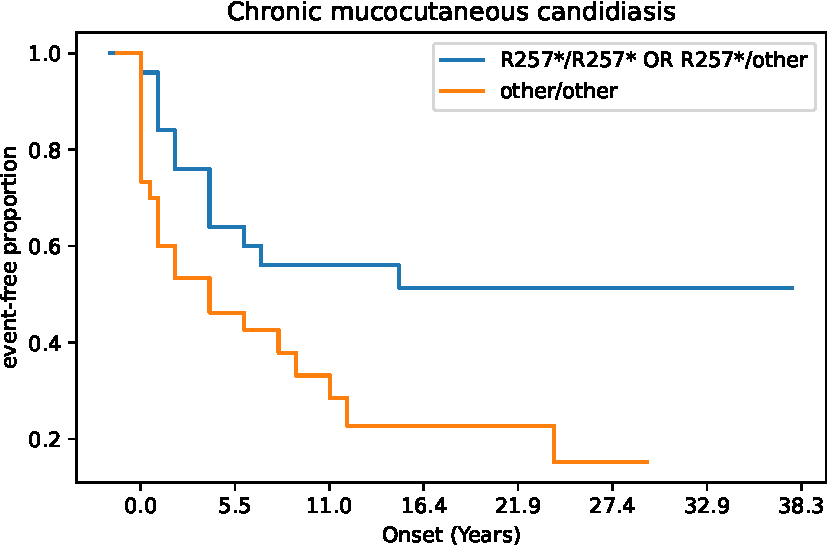
\includegraphics[width=0.3\textwidth]{ img/AIRE_cmc.pdf} 
\captionsetup{justification=raggedright,singlelinecheck=false}
\caption{log-rank p-value for Chronic mucocutaneous candidiasis (HP:0002728) and R357*/R357* or R357*/other versus other/other 0.0192}
\end{subfigure}
    
\vspace{2em}

\begin{subfigure}[b]{0.95\textwidth}
\centering
\resizebox{\textwidth}{!}{
\begin{tabular}{llllrr}
\toprule
Genotype (A) & Genotype (B) & total tests performed & significant results\\
\midrule
R257*/R257* OR R257*/other & other/other & 18 & 0\\
\bottomrule
\end{tabular}
}
\captionsetup{justification=raggedright,singlelinecheck=false}
\caption{Fisher Exact Test performed to compare HPO annotation frequency with respect to R257*/R257* OR R257*/other and other/other. }
\end{subfigure}

\vspace{2em}

\begin{subfigure}[b]{0.95\textwidth}
\captionsetup{justification=raggedright,singlelinecheck=false}
\resizebox{\textwidth}{!}{
\begin{tabular}{llllrr}
\toprule
Description & Variable & Genotype (A) & Genotype (B) & p-value & xrefs\\
\midrule
Survival analysis: Chronic mucocutaneous candidiasis & Onset of HP:0002728 & R257*/R257* OR R257*/other & other/other & 0.019 & \cite{PMID_12050215}\\
\bottomrule
\end{tabular}
}
\caption{ Onset of Chronic mucocutaneous candidiasis (HP:0002728) to compare R257*/R257* OR R257*/other and other/other with respect to Onset of HP:0002728. }
\end{subfigure}

\vspace{2em}

\caption{ The cohort comprised 58 individuals (31 females, 27 males). 2 of these individuals were reported to be deceased. A total of 47 HPO terms were used to annotate the cohort. Disease diagnosis: Autoimmune polyendocrinopathy syndrome , type I, with or without reversible metaphyseal dysplasia (OMIM:240300). A
 higher prevalence of chronic mucocutanous candidiasis with the variant Arg357Ter than with other variants was reported previously \cite{PMID_12050215}. We did not identify a significant difference in prevalence A total of 18 unique variant alleles were found in \textit{AIRE} (transcript: \texttt{NM\_000383.4}, protein id: \texttt{NP\_000374.1}).}
\end{figure}
